\section{Web Framework}\label{sec:web-framework-1}
The Web framework module handles all the connections made by external users to our service.
The framework publishes several different endpoints, as well as a Swagger documentation page of the exposed endpoints. \\ \\
The endpoints handle the basic operations of the tool, namely indexing, searching, and retrieving.
Moreover, there are two more endpoints that are used as helpers for data migration and evaluation of the system's performance.

\subsection{Indexing Endpoint}\label{subsec:indexing-endpoint-1}
The indexing endpoint (\verb|POST| \verb|/api/v1/specification|) is used to insert new OpenAPI Specifications in both MongoDB and Elasticsearch (Figure~\ref{fig:flow-index}). \\ \\
The endpoint takes an OpenAPI specification wrapped in an \verb|api| object, it extracts the natural language fields from it, and then passes it to the main pipeline.
The pipeline is composed of an embedding pipeline component -- which creates the vector embeddings for the specification, and an indexing component.
The latter is used to structure the specification in the correct way and send it both to MongoDB and to Elasticsearch.
To MongoDB, it will send the entire specification, while to Elasticsearch it will send the metadata -- if present -- together with the vector embedding of the document.

\begin{figure}[!h]
    \begin{center}
        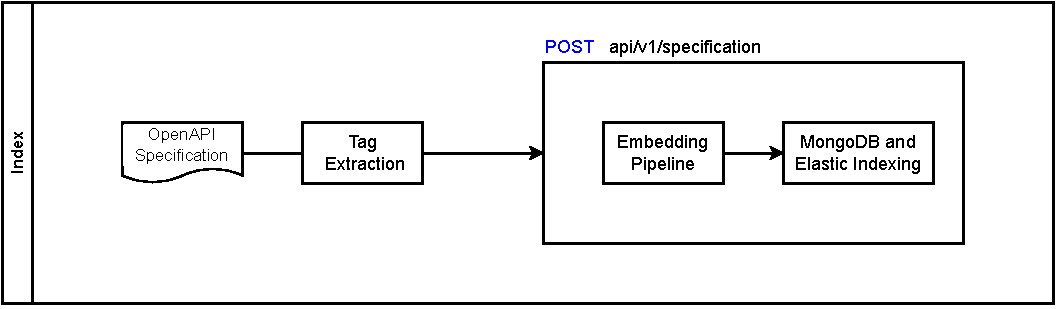
\includegraphics[width=0.8\linewidth]{assets/pdf/architecture/flow-index}
    \end{center}

    \caption{Conceptual view of the indexing pipeline}
    \label{fig:flow-index}
\end{figure}

\subsection{Search Endpoint}\label{subsec:search-endpoint-1}
In the case of the search endpoint (\verb|POST| \verb|/api/v1/search|), the user will be able to send either a specification fragment or a query, some filters, and parameters relative to the pagination and the K-NN query (Figure~\ref{fig:flow-search}).
The reason we chose a \verb|POST| request instead of a \verb|GET| request, is that the query plus the filters would have resulted in a URL that could be too long for the browser or tool to handle, thus we opted for a \verb|POST| request with a body. \\ \\
After passing a query or a specification to the endpoint, it will be preprocessed and fed to the main pipeline.
This pipeline consists of two main components, the embedding pipeline component and the DSL parsing component.
While the former creates the vector embedding from the preprocessed specification, the latter will extract the DSL field of the request and translate our DSL language into API calls that Elasticsearch uses to make its API calls.
Finally, the search query is sent to Elasticsearch, which will retrieve the most similar documents to the query.
Moreover, several calls will be made to MongoDB to retrieve the JSON specifications -- if requested by the user.

\begin{figure}[!h]
    \begin{center}
        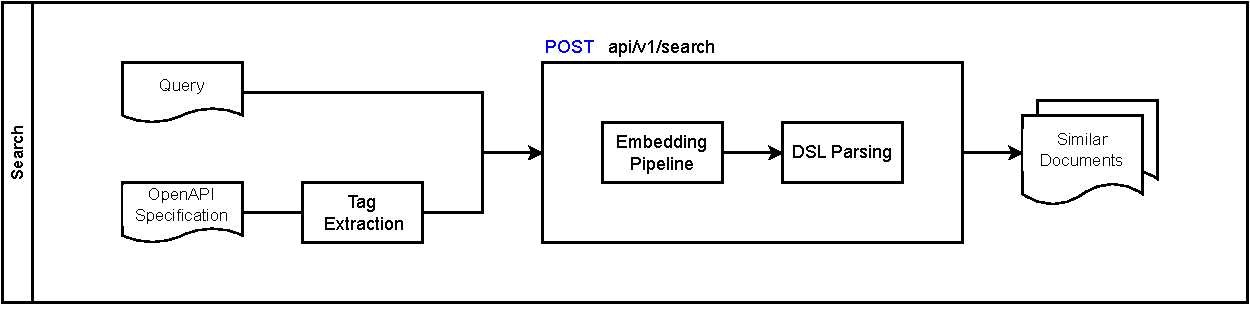
\includegraphics[width=0.9\linewidth]{assets/pdf/architecture/flow-search}
    \end{center}

    \caption{Conceptual view of the search pipeline}
    \label{fig:flow-search}
\end{figure}

\subsection{Retrieval Endpoint}\label{subsec:retrieval-endpoint-1}
The retrieval endpoint (\verb|GET| \verb|/api/v1/specification/{id}|) is used to get a specific OpenAPI Specification (Figure~\ref{fig:flow-retrieve}).
This endpoint will simply search for the given id in both the Elasticsearch and MongoDB databases, and return a document which will be a combination of the two documents returned by the two databases.

\begin{figure}[!h]
    \begin{center}
        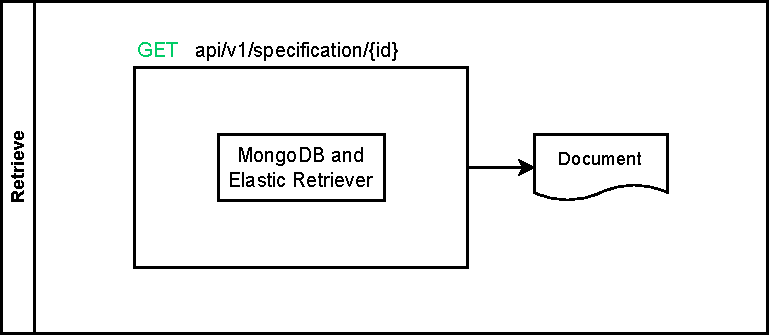
\includegraphics[width=0.5\linewidth]{assets/pdf/architecture/flow-retrieve}
    \end{center}

    \caption{Conceptual view of the retrieval pipeline}
    \label{fig:flow-retrieve}
\end{figure}

\subsection{Preprocessing Endpoint}\label{subsec:preprocessing-endpoint-1}
The preprocessing endpoint (\verb|POST| \verb|/api/v1/preprocess|) is used to simulate the preprocessing step for a search query (Figure~\ref{fig:flow-preprocess}).
This endpoint has been implemented has a helper endpoint during the evaluation process of this thesis. \\ \\
A document or query is passed as input to the endpoint.
The document will then go through the preprocessing pipeline.
In this pipeline, all the natural language tags will be extracted from the document, and then the resulting string will be cleaned of every markdown structure.
The endpoint will then return to the user a string representing the cleaned version of the input.
In a normal scenario -- i.e.\ in the case of a search or indexing query -- this string will be passed to the embedding model which will use the text to create a vector embedding for the OpenAPI Specification or query.

\begin{figure}[!h]
    \begin{center}
        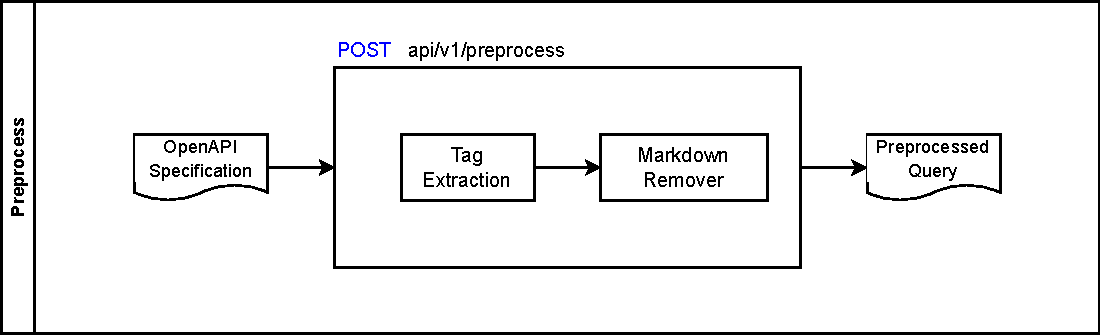
\includegraphics[width=0.8\linewidth]{assets/pdf/architecture/flow-preprocess}
    \end{center}

    \caption{Conceptual view of the preprocessing pipeline}
    \label{fig:flow-preprocess}
\end{figure}

\subsection{Synchronization Endpoint}\label{subsec:synchronization-endpoint-1}
The synchronization endpoint (\verb|PUT| \verb|/api/v1/sync|) is an idempotent endpoint used to index documents that are present in the MongoDB database in Elasticsearch (Figure~\ref{fig:flow-sync}). \\ \\
This endpoint will make sure that the two databases are always in sync.
If, while going through the MongoDB documents, it finds a document that is already in the Elasticsearch database, then it will not insert it again -- from here the idempotence and the choice of the \verb|PUT| method for this endpoint.

\begin{figure}[!h]
    \begin{center}
        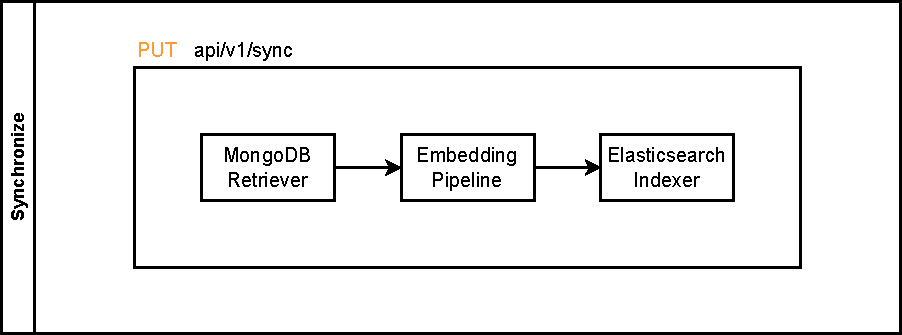
\includegraphics[width=0.7\linewidth]{assets/pdf/architecture/flow-sync}
    \end{center}

    \caption{Conceptual view of the synchronization pipeline}
    \label{fig:flow-sync}
\end{figure}
